\documentclass[12pt,a4paper]{article}
\usepackage[UTF8]{ctex}     %先引入ctex
\usepackage[utf8]{inputenc} %再引入inputenc
\usepackage{graphicx}
\usepackage{lazylatex}
\usepackage{amsmath}
\usepackage{bookmark}
\usepackage{enumerate}
\tcbuselibrary{documentation}
\graphicspath{{img/}}
% 边距
\geometry{left=2.0cm,right=2.0cm,top=2.0cm,bottom=3.0cm}
% 大题
\newenvironment{problems}{\begin{list}{}{\renewcommand{\makelabel}[1]{\textbf{##1}.\hfil}}}{\end{list}}
% 小题
\newenvironment{steps}{\begin{list}{}{\renewcommand{\makelabel}[1]{(##1)\hfil}}}{\end{list}}
% 答
\providecommand{\ans}{\textbf{答}:~}
% 解
\providecommand{\sol}{\textbf{解}.~}

% \setminted{breaklines,autogobble,frame=lines,framesep=2mm,fontsize=\scriptsize}

\usepackage{pgf-umlcd}

\begin{document}
\title{\normalsize \underline{计算机系统结构(A)}\\\LARGE 实验 3}
\author{李子龙 518070910095}
\date{\today}
\maketitle

\begin{problems}
    \item[一] \textbf{熟悉 MARS}
    \begin{steps}
        \item[1] \verb".data .word .text" 指令的含义是什么?(即:它们的用途是什么?)
         
        \ans \verb".data":标识下一个连续区块的命令都将被存储在数据段;\verb".word":列出的操作数将会被存储在数据字段为32位字;\verb".text":标识下一个连续区块的命令都将被存储在文本段。
        \item[2] 如何在 MARS 中设置断点?在第 14 行设置断点并运行至此。指令的地址是什么?
        第 14 行是否执行?
        
        \ans 在“Execute”菜单中,在14行对应的“Bkpt”打勾(如果被禁用了断点需要先按下Ctrl+T)。第14行不执行。

        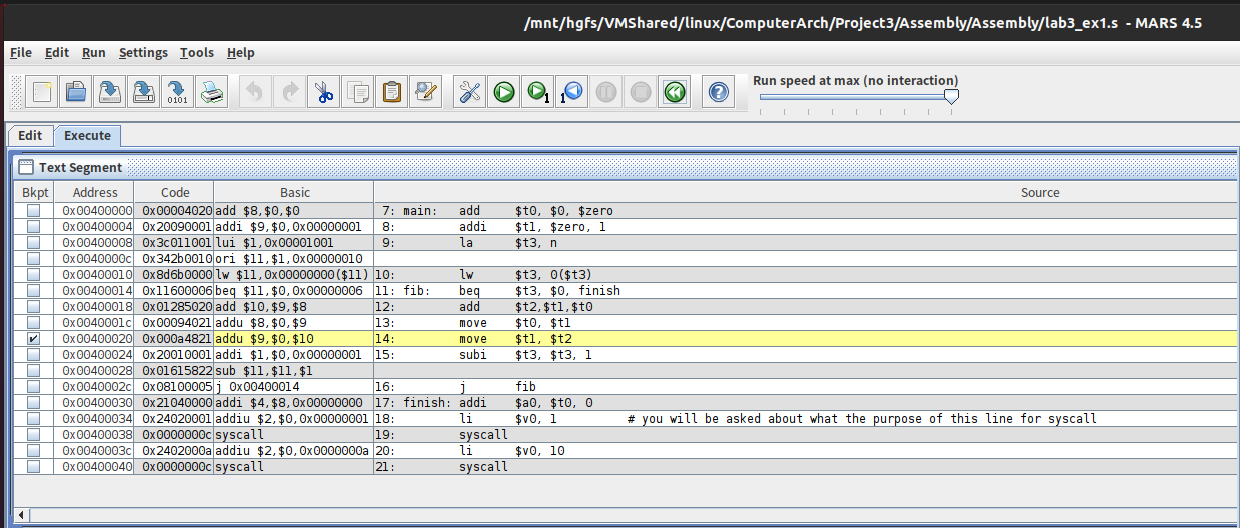
\includegraphics[width=0.9\textwidth]{bkpt.png}

        \item[3] 如果在断点处,如何继续运行你的代码?如何单步调试你的代码?将代码运行至结
        束。
        
        \ans 继续运行按下工具栏的绿色箭头,单步调试按下含有1的绿色箭头。
        \item[4] 找到 “Run I/O” 窗口 程序输出的数字是什么?如果 0 是第 0 个斐波那契数,那
        么这是第几个斐波那契数?

        \ans 34。第 9 个斐波那契数。

        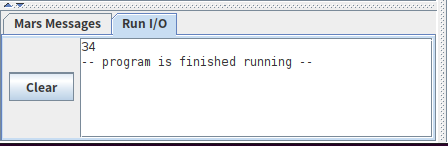
\includegraphics[width=0.6\textwidth]{run.png}
        \item[5] 在内存中, n 存储在哪个地址?尝试通过(1)查看 Data Segment ,以及(2)查看机器代码(Text Segment 中的 Code 列) 理解,如何从存储器中读取 n 。
        
        \ans n 存储在 \verb"0x10010010" 地址。

        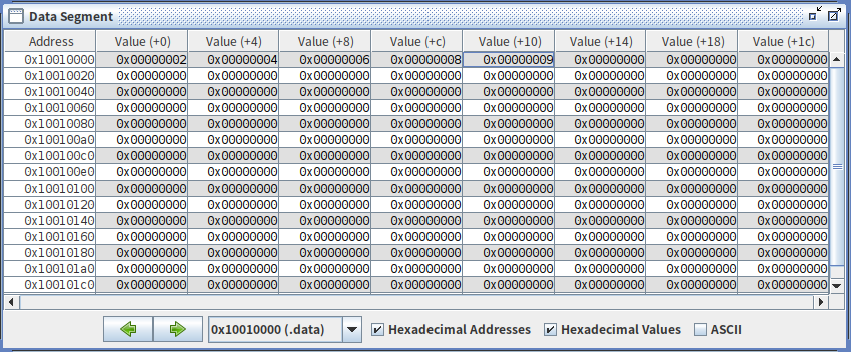
\includegraphics[width=0.7\textwidth]{ds.png}

        所谓的
        \begin{verbatim}
            la  $t3, n
        \end{verbatim}
        伪指令被翻译为 MIPS 指令
        \begin{verbatim}
            lui $l, 0x00001001
            ori $ll, $l, 0x00000010
        \end{verbatim}

        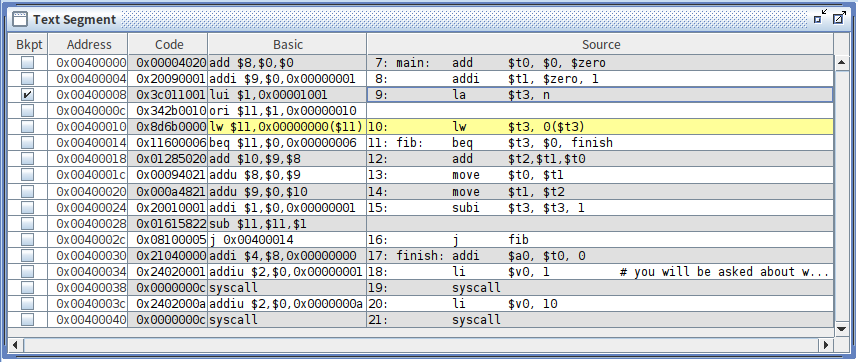
\includegraphics[width=0.7\textwidth]{ts.png}

        第一条指令将 \verb"0x00001001" 地址送至寄存器高位 \verb"$at" 的前16位中;第二条指令将上面的地址与0x00000010做或运算存放到临时变量寄存器 \verb"$t3" 中,这样就将 n 的地址取出放在了 \verb"$t3"。

        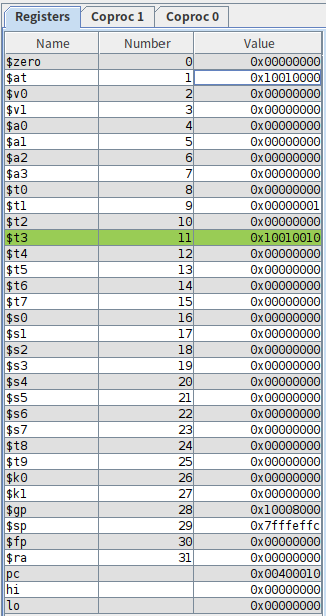
\includegraphics[width=0.3\textwidth]{reg.png}
        \item[6] 如何在不改变“Edit”栏 下的代码的条件下,通过在执行前手动修改存储位置的值,
        让程序计算第 13 个斐波那契数(索引从 0 开始)? 你可以取消勾选 Data Segment
        底部的 “Hexadecimal Values” 框方便观察。

        \ans 直接将代码区的对应的内存数值修改即可,得到233:

        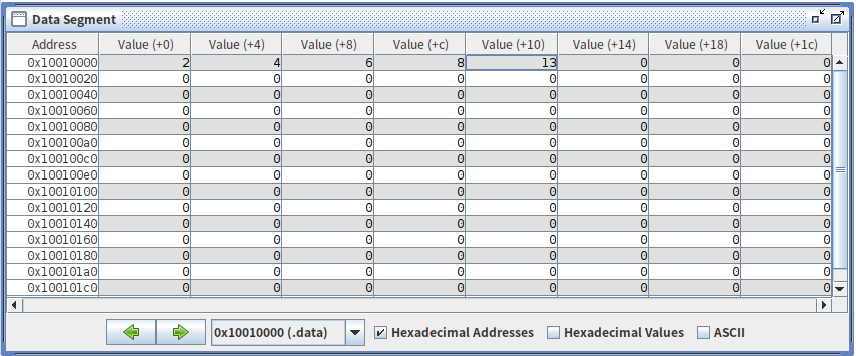
\includegraphics[width=0.8\textwidth]{dsf.png}

        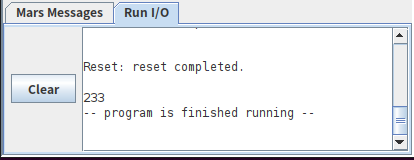
\includegraphics[width=0.6\textwidth]{run13.png}
        \item[7] 如何观察和修改一个寄存器中的值?重置模拟( Run $\rightarrow$ Reset )并通过 (1)在一个
        设置好的断点停下,(2)只修改一个寄存器 (3)解除断点,来计算第 13 个斐波
        那契数。
        第 19 行和第 21 行用到了 \texttt{syscall} 指令。它是什么?如何使用它?(提示:可以查看 MARS 的 Help 菜单)

        \ans 在第 10 行处设置断点,当该行单步运行结束后,修改寄存器 \verb"$t3" 的值为 13,取消断点,继续运行。会得到相同的 233 结果。

        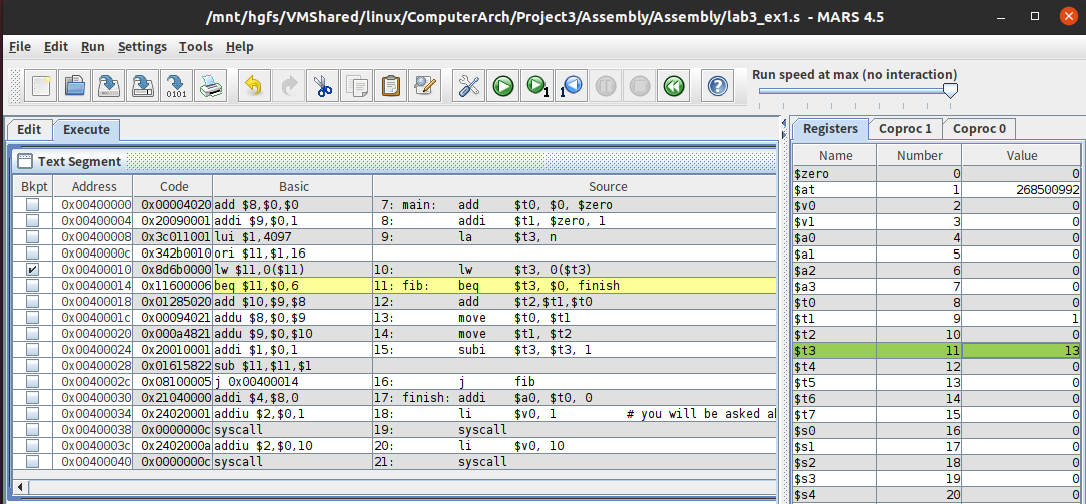
\includegraphics[width=0.8\textwidth]{fixreg.png}

        第19行时,寄存器\verb"$v0"的值被设置为1,对应的\verb"syscall"的模式为打印寄存器\verb"$a0"的整数:34. 第21行时,寄存器\verb"$v0"的值已经被设置为10,对应的\verb"syscall"的模式为退出。
    \end{steps} 
    \item[二] \textbf{将 C 编译为 MIPS}
    \begin{steps}
        \item[1] 在生成的 MIPS 汇编代码 lab3\_ex2.s 中 找到将 source 复制到 dest 的循环部分所
        对应的指令。

        循环部分对应的指令:
        \begin{code}{asm}
$L3:
    sw	$4,0($3)
    lw	$4,0($2)
    addiu	$3,$3,4
    addiu	$2,$2,4
    bne	$4,$0,$L3
    nop
        \end{code}
        
        \item[2] 找到 lab\_ex2.c 中的 source 和 dest 指针最初在汇编文件中存储的位置。 最后,解释这些指针是如何通过循环进行操作的。
        
        \begin{verbatim}
        lui	$3,%hi(dest)
        lui	$2,%hi(source+4)
        addiu	$3,$3,%lo(dest)
        addiu	$2,$2,%lo(source+4)
        \end{verbatim}

        source 指针被存放在 \verb"$2" 中(+4是为了对齐),dest 指针被存放在 \verb"$3" 中。

        首先会将 dest 指针的地址从 \verb"$3" 取出存放在 \verb"$4" 中,之后会将 \verb"$4" 地址所对应的值设置为 source 对应的 \verb"$2" 地址指向的值。之后两个指针地址寄存器+4,准备读取下一个数。现在 \verb"$4" 已经是之前的 dest 和 source 对应的值,如果它不等于 0 就会循环,否则会到下面的 \verb"$L2" 标签区域。

    \end{steps}
    \item[三] \textbf{函数调用的过程}
    
    需要保存 \verb"$s0 $s1 $s2 $ra"寄存器变量到栈帧中。
    \begin{code}{asm}
nchoosek:
	# prologue
	### YOUR CODE HERE ##
	addi	    $sp, $sp, -16
	sw	        $ra, 12($sp)
	sw	        $s2, 8($sp)
	sw	        $s1, 4($sp)
	sw	        $s0, 0($sp)
    \end{code}

    \begin{code}{asm}
return:
	# epilogue
	### YOUR CODE HERE ###
	lw	    $s0, 0($sp)
	lw	    $s1, 4($sp)
	lw	    $s2, 8($sp)
	lw	    $ra, 12($sp)
	addi        $sp, $sp, 16
	jr 	    $ra
    \end{code}

    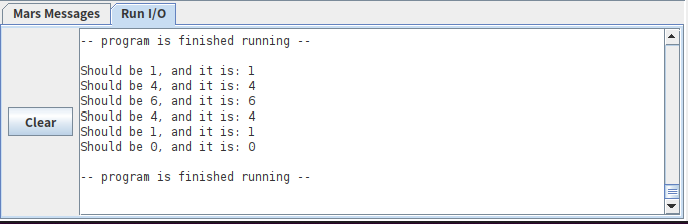
\includegraphics[width=0.8\textwidth]{ex3.png}

\end{problems}


\end{document}
